% === GO TO THE USER CUSTOMIZATION SECTION TO MAKE CHANGES

\documentclass[article, a4paper, 12pt, ]{memoir}

% Please use XeLaTeX to compile

\usepackage{xltxtra}
\defaultfontfeatures{Ligatures=TeX}
\usepackage{hyphenat}

\newcommand\setlogofont[1]{\newfontfamily\logofont{#1}}
\newcommand\setlicensefont[1]{\newfontfamily\licensefont{#1}}
\usepackage{microtype}
\usepackage{rotating}
\usepackage{hyperxmp}
\usepackage[colorlinks=true, unicode=true, breaklinks=true, linkcolor=black, urlcolor=blue, citecolor=black]{hyperref}

\counterwithout{section}{chapter}
\setsecnumdepth{subsubsection}
\setcounter{tocdepth}{3}

\usepackage[export]{adjustbox}
\usepackage{graphicx}
\usepackage[type={CC}, modifier={by}, version=4.0]{doclicense}

\newcommand\affiliation[1]{{\normalfont\normalsize\itshape#1}}

\pagestyle{simple}
\makeevenfoot{simple}{}{}{}
\makeoddfoot{simple}{}{}{}
\raggedbottom

\newcommand\authorheader[1]{\makeevenhead{simple}{\footnotesize\itshape#1}{}{\footnotesize\thepage}}
\newcommand\titleheader[1]{\makeoddhead{simple}{\footnotesize\thepage}{}{\footnotesize\itshape#1}}

\newcommand\thisdoi{10.1010/1010101010101010101010}
\newcommand\thisdoilink{https://doi.org/\thisdoi}

\renewcommand{\maketitlehooka}{%
  \vspace*{-60pt}
  \noindent\hspace*{-25pt}\begin{minipage}[t]{2.5cm}
    \vspace*{-16pt}
    
\includegraphics[valign=t, width=2.5cm]{pihph-logo.png}
  \end{minipage}
  \begin{minipage}[t]{.75\linewidth}
    \centering
    \logofont\Large Papers in Historical Phonology\\[5pt]

    \footnotesize

    http://journals.ed.ac.uk/pihph

    ISSN 2399-6714

    \footnotesize\vspace*{5pt}

    Volume 1, \thepage--\thelastpage

    DOI: \href{\thisdoilink}{\thisdoi}
  \end{minipage}
  \begin{minipage}[t]{2.1cm}
    \centering
    \vspace*{-14pt}
    \adjustbox{valign=t}{\doclicenseImage[imagewidth=2.1cm]}\\
      \licensefont\tiny Licensed under~a \doclicenseLongNameRef{} License
  \end{minipage}
}

\pretitle{\vspace*{24pt}\begin{center}\large\bfseries}
\preauthor{\begin{center}\large\scshape\begin{tabular}[t]{c}}
\postauthor{\end{tabular}\end{center}\vspace*{12pt}}
\predate{\relax}
\postdate{\relax}
\date{}

\captionnamefont{\footnotesize\bfseries}
\captiontitlefont{\footnotesize}

\renewcommand\abstractnamefont{\normalfont\footnotesize\bfseries}
\renewcommand\abstracttextfont{\normalfont\footnotesize}
\setlength\absleftindent{1cm}
\setlength\absrightindent{1cm}
\setlength{\abstitleskip}{-17pt}
\setbeforesecskip{-18pt}
\setaftersecskip{6pt}
\setsecheadstyle{\normalfont\bfseries}
\setbeforesubsecskip{-18pt}
\setaftersubsecskip{6pt}
\setsubsecheadstyle{\normalfont\bfseries}
\setbeforesubsubsecskip{-18pt}
\setaftersubsubsecskip{6pt}
\setsubsubsecheadstyle{\normalfont\bfseries}
\renewenvironment{quote}{\list{}{\leftmargin=0.7cm\rightmargin=0.7cm}\item[]\footnotesize}{\endlist}

\setlrmarginsandblock{4cm}{4cm}{*}
\setulmarginsandblock{4.5cm}{4.5cm}{*}
\checkandfixthelayout

\setlength{\footmarkwidth}{0em}
\setlength{\footmarksep}{0em}
\footmarkstyle{\textsuperscript{#1}\hspace{.3em}}
\setfootins{24pt}{\bigskipamount}
\renewcommand*{\footnoterule}{%
   \kern-3pt%
   \hrule width 0.4\columnwidth
   \kern 2.6pt
 \vspace{12pt}}

\usepackage[usenames]{xcolor}
\definecolor{pihphgreen}{RGB}{118, 146, 60}
\usepackage[most]{tcolorbox}

\newtcolorbox{tcdoublebox}[1][]{%
  enhanced jigsaw,
  sharp corners,
  colback=white,
  text width=.95\textwidth,
  before={\vspace*{18pt}\noindent},
  left skip=-5mm,
  borderline={1pt}{-2pt}{black},
  #1
}

\newcommand\commentsinvited{
\begin{tcdoublebox}

\section*{\textcolor{pihphgreen}{Comments invited}}

\textit{PiHPh} relies on post-publication review of the papers that it publishes. If you have any comments on this piece, please add them to its comments site. You are encouraged to consult this site after reading the paper, as there may be comments from other readers there, and replies from the author. This paper's site is here:

\noindent \url{\thisdoilink}

\end{tcdoublebox}
}

\widowpenalty=10000
\clubpenalty=10000

% === START OF USER CUSTOMIZATION


\title{Modelling frequency effects in sound change chains}
\author{Stefano Coretta\\\affiliation{The University of Manchester}}

\authorheader{Stefano Coretta}
\titleheader{Modelling frequency effects in sound change chains}

\setmainfont{Cambria} % If you do not have access to Cambria, you can use the metric-equivalent Caladea: https://fontlibrary.org/en/font/caladea
\setlicensefont{Calibri} % If you do not have access to Calibri, you can use the metric-equivalent Carlito: https://fontlibrary.org/en/font/carlito
\setlogofont{Lekton} % Available at https://www.fontsquirrel.com/fonts/lekton

% If any of these fonts are not available on your system, feel free to
% change them here, but of course the final layout will then differ

\usepackage{polyglossia}                   % or use babel if desired
\setmainlanguage[variant=british]{english} % or use babel if desired
\usepackage[autostyle, english=british]{csquotes} % remove the english=british option for double quotes
\usepackage{expex} % for examples, feel free to use anything else


% Some recommended packages

\usepackage{booktabs} % for nice tables

% BibTeX setup, deprecated
\usepackage{natbib}
\bibpunct[:]{(}{)}{;}{a}{}{,}
\setlength\bibsep{0pt}


\begin{document}
\setcounter{page}{1}
\maketitle


\section{Methods}\label{methods}

Four simulations were implemented in R \citep{r-core-team2017} to test
the behaviour of the model described in \ldots{} The simulation starts
with the creation of a lexicon of 100 lexical items. 50 words are
assigned to the BART category, while the remaining 50 to the BAT
category. Within each category, lexical frequency from 1 to 50 is
assigned to each lexical item, so that there are a BART and a BAT word
of frequency 1, a BART and a BAT word of frequency 2, etc. The lexicon
is then populated using the specified formant values (6.5 and 5.5 Bark
in this simulation). A loop produces 50,000 total tokens among the
lexical items. The selection of the items is randomised and the weight
of each item depends on its lexical frequency. Higher frequency items
(words) have thus more tokens in their representation than lower
frequency words.

After the lexicon is initialised, a simulated sound change is applied to
such lexicon. The simulation goes through 200,000 iterations, in each of
which a random lexical item is selected (lexical frequency weighing
applies) and produced. To produce the selected lexical item, a random
target among the exemplars is chosen and produced with a random level of
noise (here between -0.2 and +0.2). If the selected word is a word
containing the vowel which is undergoing change (the biased vowel), then
a bias of -0.3 is applied to the formant value (on top of the noise).

Now that the word has been produced, an algorithm decides weather the
word will be encoded back in memory or disregarded. This will depend on
its lexical frequency and most importantly on whether the token falls in
an area of ambiguity, as in \citep{hay2015}. If the token is not
ambiguous, i.e.~if it is surrounded only by tokens of the same category,
then the probability of being encoded back in memory is set to 1 (such a
word is always sent back to memory). If the token is ambiguous, i.e.~if
it falls in an area of overlap containing tokens of both categories,
then the probability of being encoded in memory is set as a function of
the lexical frequency of the relative word: p(x\textbar{}M) =
frequency(x) / maximum(frequency).

Once a word has been encoded in memory (or not, depending on the outcome
of the encoding function), a new cycle of the algorithm begins and
another word is chosen, produced and encoded (or not).

\subsection{Statistical analysis}\label{statistical-analysis}

Generalised additive mixed model are used for statistical analysis.

\section{Results}\label{results}

\begin{figure}
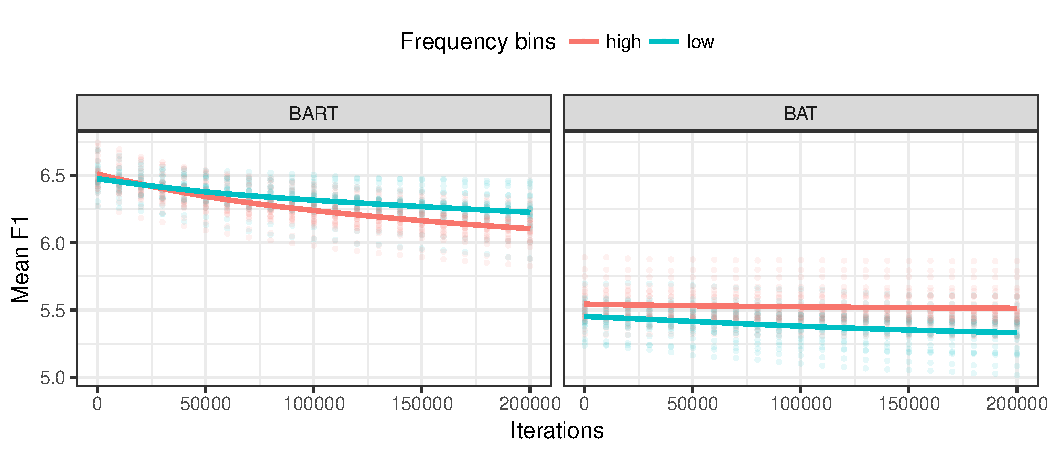
\includegraphics{../../figures/plot_1.pdf}
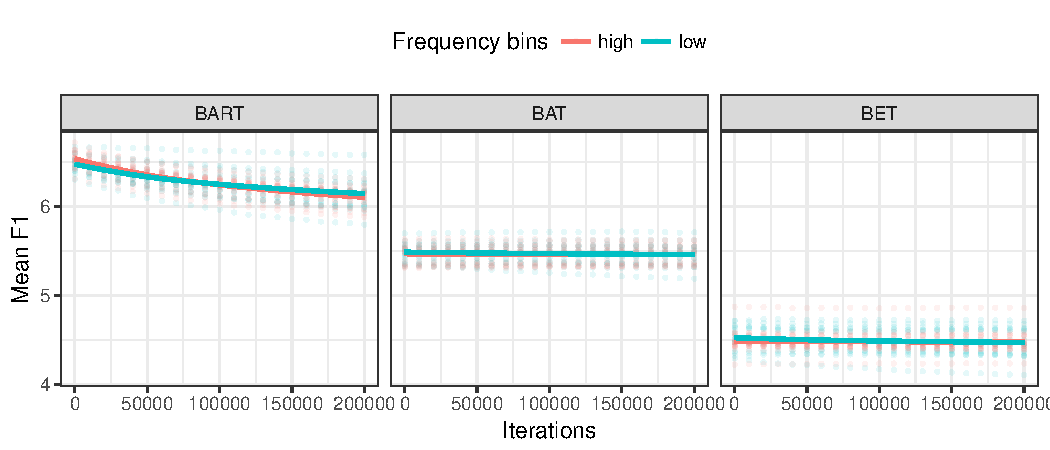
\includegraphics{../../figures/plot_2.pdf}
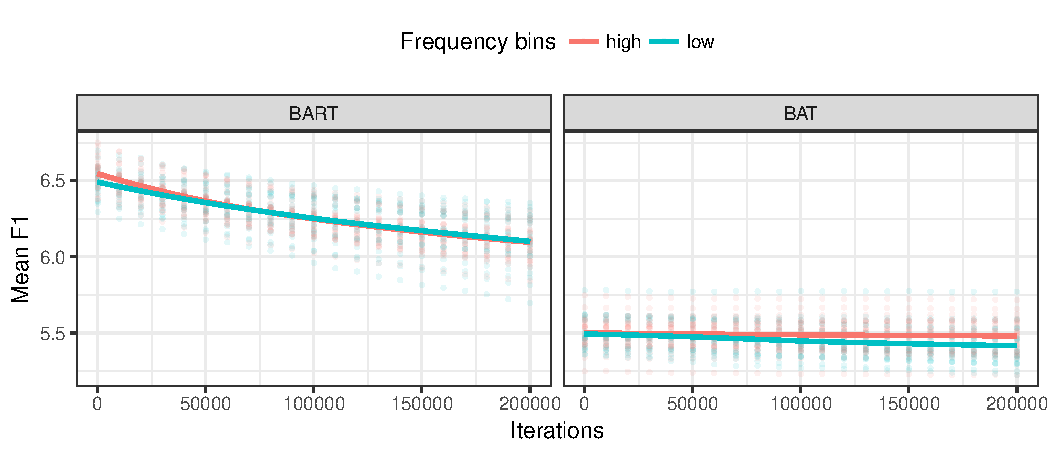
\includegraphics{../../figures/plot_3.pdf}
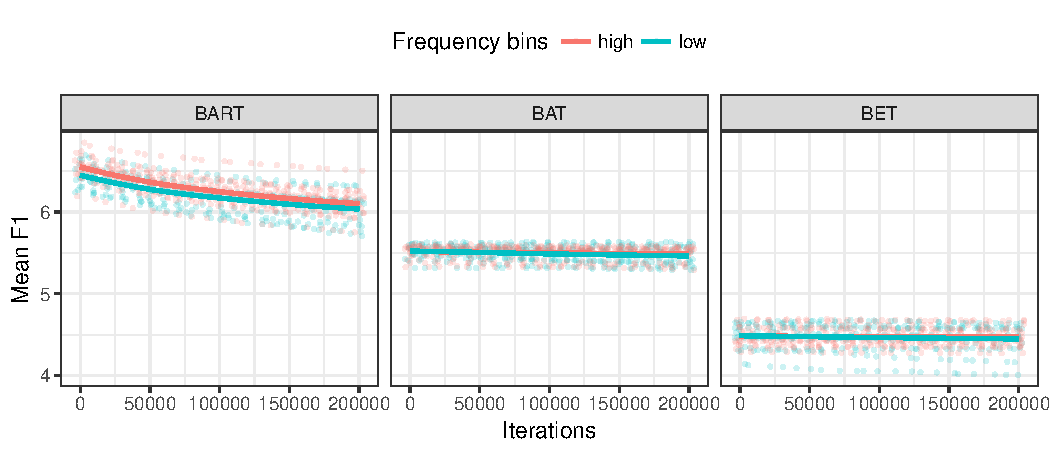
\includegraphics{../../figures/plot_4.pdf}
\caption{Change in F3.}
\label{f:results}
\end{figure}

Starting from simulation 1, a general trend of decreasing mean F1
through time can be observed both in BART and BAT words, as shown in the
top panel of \Cref{f:results}. The graph also shows the decrease of mean
F1 for low and high frequency words separately. The frequency bins were
defined as the lower half (1--25) and upper half (26--50) of the
frequency range (1--50). Mean F1 decreases at a higher rate in low
frequency than in high frequency words in BAT words. The model in
\ldots{} thus correctly pushes low frequency words faster, as it was
supposed to. Unexpectedly, though, it is high frequency words that
change at a higher rate in BART words, not low frequency words. The
model in its current state thus predicts that the effect of frequency on
chain sound changes differs depending whether the observed phonetic
category is the pushing category or the pushed category.

This pattern can be observed also in simulations 2 to 4. High frequency
words change faster in the pushed category (BART), but low frequency
ones do in the pushed category (BAT) or categories if there is more than
one (BAT, BET). The main qualitative difference in these simulations if
compared to simulation 1 is the magnitude of the effect of frequency,
which is smaller. Simulations 2 and 4 also clearly show that both pushed
categories (BAT, BET) undergo the effect of lexical frequency.

\commentsinvited % Please do not change this



\section*{Author's contact details}
\label{sec:auth-cont-deta}

\noindent \textit{Stefano Coretta}

\noindent The University of Manchester

\vspace*{5pt}
\noindent \textit{\href{mailto:stefano.coretta@manchester.ac.uk}{\nolinkurl{stefano.coretta@manchester.ac.uk}}}


% BibTeX setup, deprecated
\bibliographystyle{unified} % unified.bst can be obtained at http://cexlj.org/downloads/unified.bst
\renewcommand\bibsection{\section*{References}}
\bibliography{linguistics.bib}

\end{document}
